\section{Results}
\label{sec:results}

\subsection{Frontier LLM Persona Convergence}
\label{sec:results_survey}

Our survey of GPT-4o, GPT-4o-mini, and GPT-4.1-mini confirms the persona collapse phenomenon. \Tabref{tab:survey} shows that 7 out of 10 preference questions elicit unanimous convergence across all three model variants. All models prefer chocolate lava cake, the color blue, dolphins, the number 7, and early morning---despite being independently fine-tuned. The remaining three questions show 2/3 agreement, with the only divergence on seasonal preference (autumn vs.\ spring) and planet preference (Mars vs.\ Saturn). When asked about programming languages, all three models refuse to commit, instead answering ``it depends''---itself a form of convergent attractor behavior.

\begin{table}[t]
\centering
\caption{Frontier LLM persona convergence. We query three GPT-4o family models with preference questions (5 samples each at temperature 0.7). Agreement indicates the number of models sharing the top response.}
\label{tab:survey}
\begin{tabular}{@{}lll@{}}
\toprule
\textbf{Question} & \textbf{Convergent Response} & \textbf{Agreement} \\
\midrule
Favorite dessert? & Chocolate lava cake & \textbf{3/3} \\
Preferred color? & Blue & \textbf{3/3} \\
Favorite animal? & Dolphins & \textbf{3/3} \\
Favorite number? & 7 & \textbf{3/3} \\
Time of day? & Early morning & \textbf{3/3} \\
Best way to learn? & Active engagement & \textbf{3/3} \\
Programming language? & ``Depends'' (refuses) & \textbf{3/3} \\
Best season? & Autumn / Spring & 2/3 \\
Most interesting planet? & Mars / Saturn & 2/3 \\
\bottomrule
\end{tabular}
\end{table}

\subsection{Training Performance}
\label{sec:results_training}

At the small scale (${\sim}4$M parameters), the \transformer and \gru achieve nearly identical validation perplexity (28.3 vs.\ 28.6), while \lstm lags substantially (48.1). This near-parity between Transformer and GRU at small scale is critical: it allows us to attribute differences in default behavior to architectural inductive biases rather than capability gaps. At the medium scale (${\sim}10$M parameters), all models are undertrained relative to their capacity due to the limited training corpus (2.6M tokens), with perplexities of 31.6, 41.3, and 91.8 respectively. Training curves are shown in \figref{fig:training}.

\begin{figure}[t]
\centering
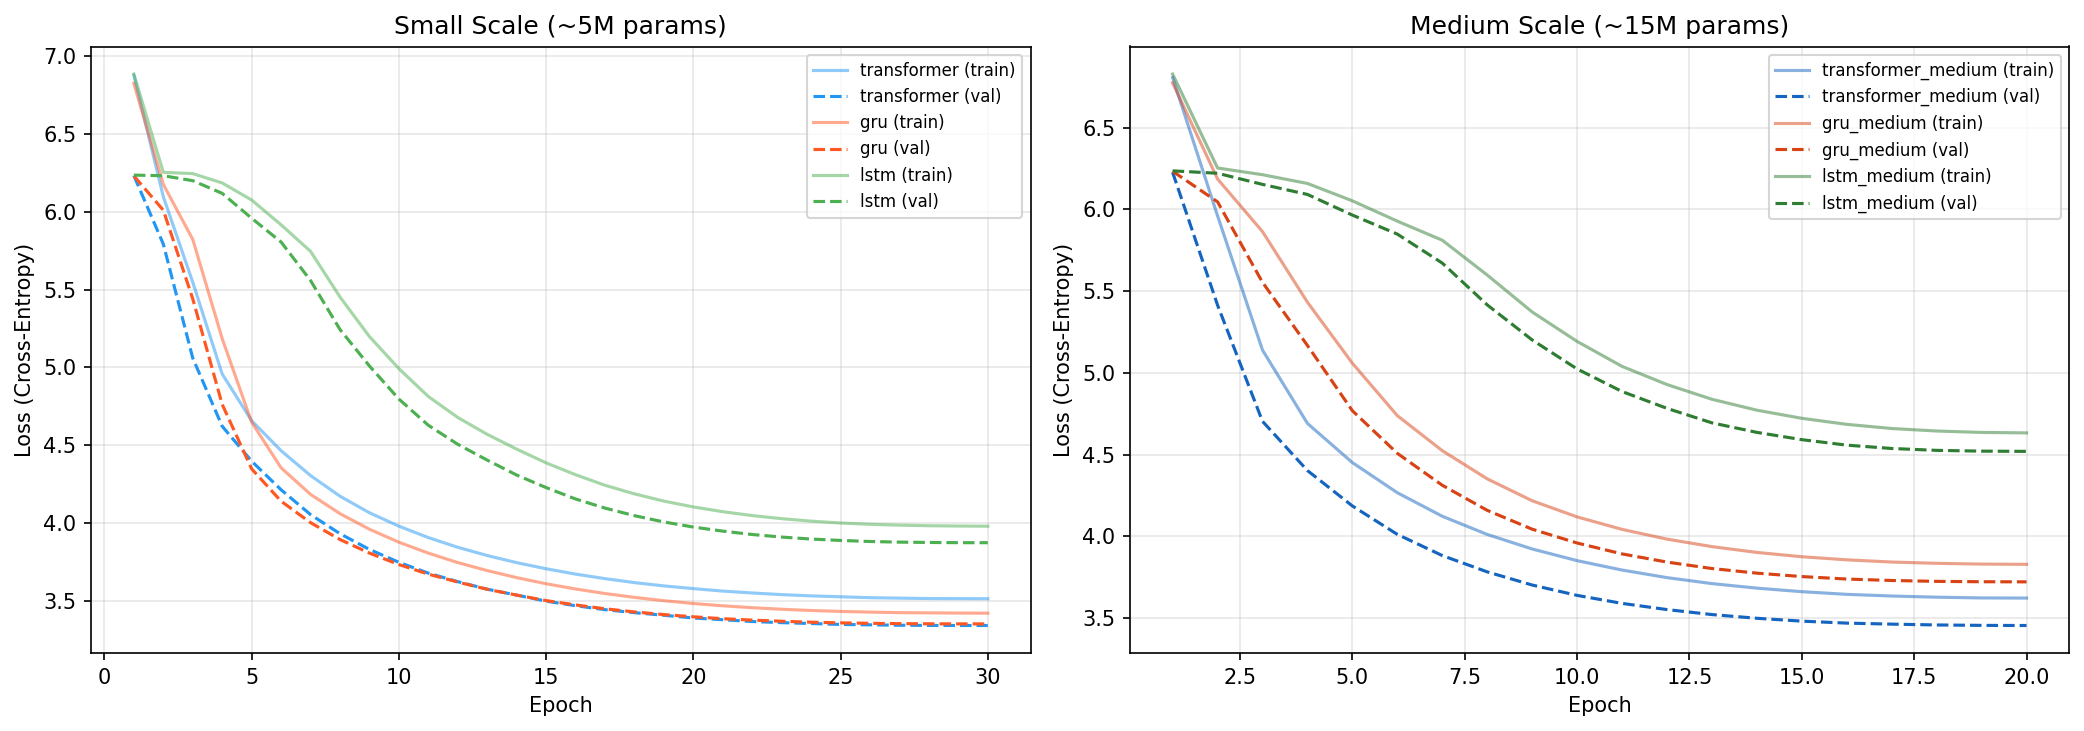
\includegraphics[width=0.95\linewidth]{figures/training_curves.png}
\caption{Training loss curves for all six models. At small scale, \transformer and \gru converge to similar final loss (${\sim}3.35$), while \lstm plateaus higher. Medium-scale models are undertrained relative to their capacity.}
\label{fig:training}
\end{figure}

\subsection{Response Diversity}
\label{sec:results_diversity}

\Tabref{tab:entropy} reports the mean Shannon entropy of generated content words across 20 completions per prompt. All architectures produce diverse completions, but with consistent ordering: \transformer produces slightly more diverse responses than \gru, while \lstm is consistently the least diverse. The difference between \transformer and \gru is not statistically significant (Mann-Whitney $U$, $p = 0.70$), but the \transformer vs.\ \lstm comparison shows a moderate effect size (Cohen's $d = 0.38$).

\begin{table}[t]
\centering
\caption{Response entropy (bits) across architectures. Higher entropy indicates more diverse completions. The \transformer--\gru difference is not significant ($p = 0.70$); the \transformer--\lstm difference shows moderate effect (Cohen's $d = 0.38$).}
\label{tab:entropy}
\begin{tabular}{@{}lcc@{}}
\toprule
\textbf{Model} & \textbf{Small (entropy)} & \textbf{Medium (entropy)} \\
\midrule
\transformer & 2.882 & \textbf{2.960} \\
\gru & \textbf{2.878} & 2.913 \\
\lstm & 2.552 & 2.794 \\
\bottomrule
\end{tabular}
\end{table}

An analysis of the most frequent content words reveals qualitative differences in what each architecture defaults to. \transformer and \lstm both show a strong female-protagonist bias (``she'', ``her'' as top words), while \gru favors group-oriented language (``they'', ``had''). All architectures share ``big'' and ``day'' among their top content words, reflecting shared training data rather than architectural preference.

\subsection{Representation-Level Attractor Structure}
\label{sec:results_representation}

\Figref{fig:representation} and \tabref{tab:representation} present the representation analysis across 25 prompts in 5 semantic categories.

\begin{table}[t]
\centering
\caption{Representation-level attractor structure. Within-concept and between-concept similarity are measured by cosine similarity of hidden states. Concept separation is their difference (positive = concepts are distinguishable). Attractor basin size is the mean Euclidean distance to category centroids (smaller = tighter attractor).}
\label{tab:representation}
\begin{tabular}{@{}lcccc@{}}
\toprule
\textbf{Architecture} & \textbf{Within-Concept} & \textbf{Between-Concept} & \textbf{Concept Sep.} & \textbf{Basin Size} \\
\midrule
\transformer & 0.943 & 0.950 & $-0.007$ & \textbf{4.37} \\
\gru & 0.839 & 0.863 & $-0.024$ & 7.63 \\
\lstm & 0.854 & 0.794 & \textbf{+0.060} & 6.97 \\
\bottomrule
\end{tabular}
\end{table}

The results reveal a striking pattern. \transformer has the tightest overall representation space (within-concept similarity 0.943, basin size 4.37) but the worst concept separation ($-0.007$). Everything maps to a similar region of hidden space---food prompts, animal prompts, color prompts, and emotion prompts all land within a narrow band of cosine similarity. We call this a \emph{universal attractor basin}: the Transformer attention mechanism creates representations where all inputs converge toward a shared region, regardless of semantic content.

\lstm, despite its lower overall capability (perplexity 48.1 vs.\ 28.3), maintains the best concept separation ($+0.060$). The LSTM's gating mechanism and fixed-size cell state force information-theoretic trade-offs that preserve distinct representations for different semantic categories. \gru falls between the two, with moderate similarity values and negative concept separation ($-0.024$).

\begin{figure}[t]
\centering
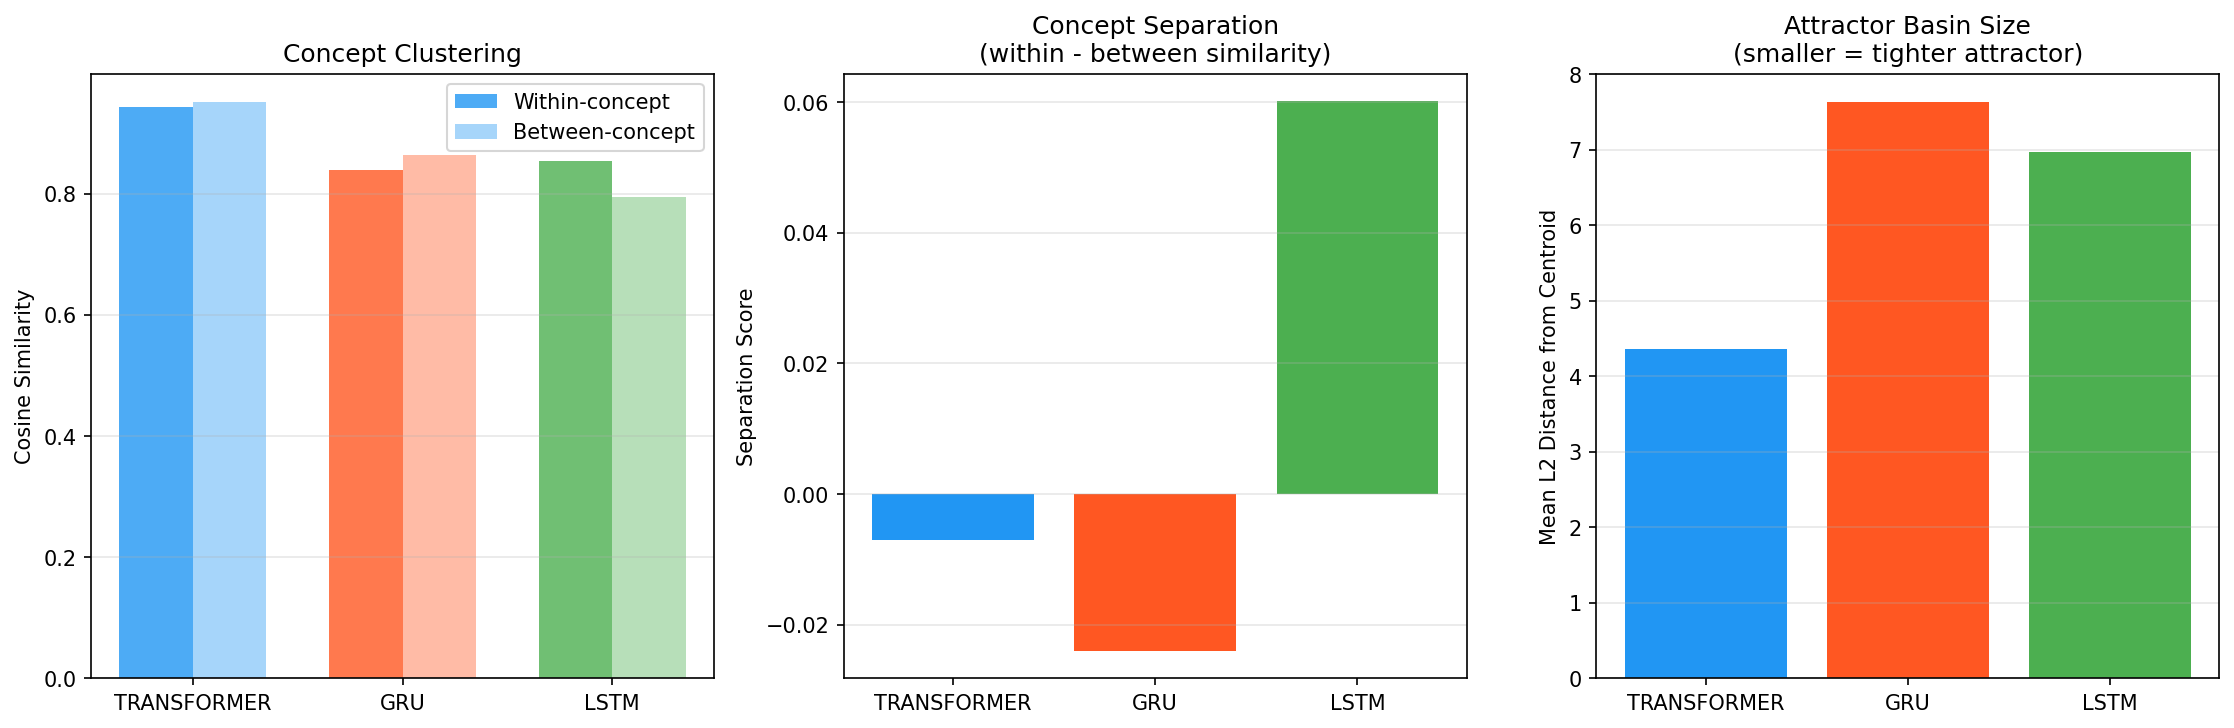
\includegraphics[width=0.95\linewidth]{figures/representation_analysis.png}
\caption{Representation structure across architectures. \transformer creates a uniformly tight representation space where all concepts cluster together (universal attractor basin). \lstm maintains distinct concept clusters despite lower overall capability.}
\label{fig:representation}
\end{figure}

\subsection{Next-Word Attractor Analysis}
\label{sec:results_nextword}

This experiment provides the most direct evidence that architectures develop different default responses. We compare top-1 next-word predictions across architectures for 12 prompts.

\para{Top-1 agreement rate: 25\%.} Only 3 out of 12 prompts produce the same greedy prediction across all three architectures. \Tabref{tab:nextword} shows representative examples. For the prompt ``she was very \_\_\_'', \transformer predicts ``excited'' (12.5\%), \gru predicts ``happy'' (19.4\%), and \lstm predicts ``years'' (8.0\%---a degenerate response reflecting its lower capability). For ``the little girl named \_\_\_'', \transformer concentrates 43.3\% of probability mass on ``lily.'', while \gru spreads more evenly with 26.8\% on ``lily'' and \lstm defaults to ``a'' (62.0\%).

\begin{table}[t]
\centering
\caption{Next-word predictions across architectures. Each cell shows the top-1 prediction and its probability. Prompts where all architectures agree are marked with $\dagger$.}
\label{tab:nextword}
\resizebox{\textwidth}{!}{%
\begin{tabular}{@{}llll@{}}
\toprule
\textbf{Prompt} & \textbf{\transformer} & \textbf{\gru} & \textbf{\lstm} \\
\midrule
``she was very \_\_\_'' & excited (12.5\%) & happy (19.4\%) & years (8.0\%) \\
``in the forest there was a friendly \_\_\_'' & boy (6.1\%) & girl (10.1\%) & old (7.9\%) \\
``the little girl named \_\_\_'' & lily. (43.3\%) & lily (26.8\%) & a (62.0\%) \\
``the little boy had a pet \_\_\_'' & dog (25.6\%) & cat (13.4\%) & . (14.2\%) \\
$\dagger$ ``he wanted to \_\_\_'' & play (25.6\%) & play (18.6\%) & play (31.6\%) \\
$\dagger$ ``her favorite color was \_\_\_'' & pink (18.3\%) & pink (15.7\%) & pink (21.1\%) \\
``they decided to \_\_\_'' & play (25.6\%) & go (18.6\%) & play (31.6\%) \\
\bottomrule
\end{tabular}
}
\end{table}

\para{Jensen-Shannon divergence.} \Tabref{tab:jsd} reports the mean $\jsd$ between full next-word distributions for each architecture pair. Architecturally closer models (\transformer--\gru) show lower divergence (0.339) than more distant pairs (\gru--\lstm: 0.505). The highest per-prompt divergence occurs for ``the little girl named \_\_\_'' ($\jsd = 0.798$), where architectures disagree most sharply. The lowest divergence occurs for ``he wanted to \_\_\_'' ($\jsd = 0.217$), where the training data dominates and all architectures converge on ``play''---reflecting children's stories rather than architectural preference.

\begin{table}[t]
\centering
\caption{Mean Jensen-Shannon divergence between next-word distributions across 12 prompts. Lower values indicate more similar output distributions.}
\label{tab:jsd}
\begin{tabular}{@{}lc@{}}
\toprule
\textbf{Architecture Pair} & \textbf{Mean $\jsd$} \\
\midrule
\transformer vs.\ \gru & \textbf{0.339} \\
\transformer vs.\ \lstm & 0.480 \\
\gru vs.\ \lstm & 0.505 \\
\bottomrule
\end{tabular}
\end{table}

\para{Transformer attractor sharpness.} A consistent pattern across prompts is that \transformer concentrates more probability mass on its top prediction than \gru does. For ``the little girl named \_\_\_'', \transformer puts 43.3\% on a single token while \gru puts 26.8\%. This sharper probability peak means the Transformer's attractor has a steeper basin---once it begins to prefer a response, it commits more strongly than the GRU.

\begin{figure}[t]
\centering
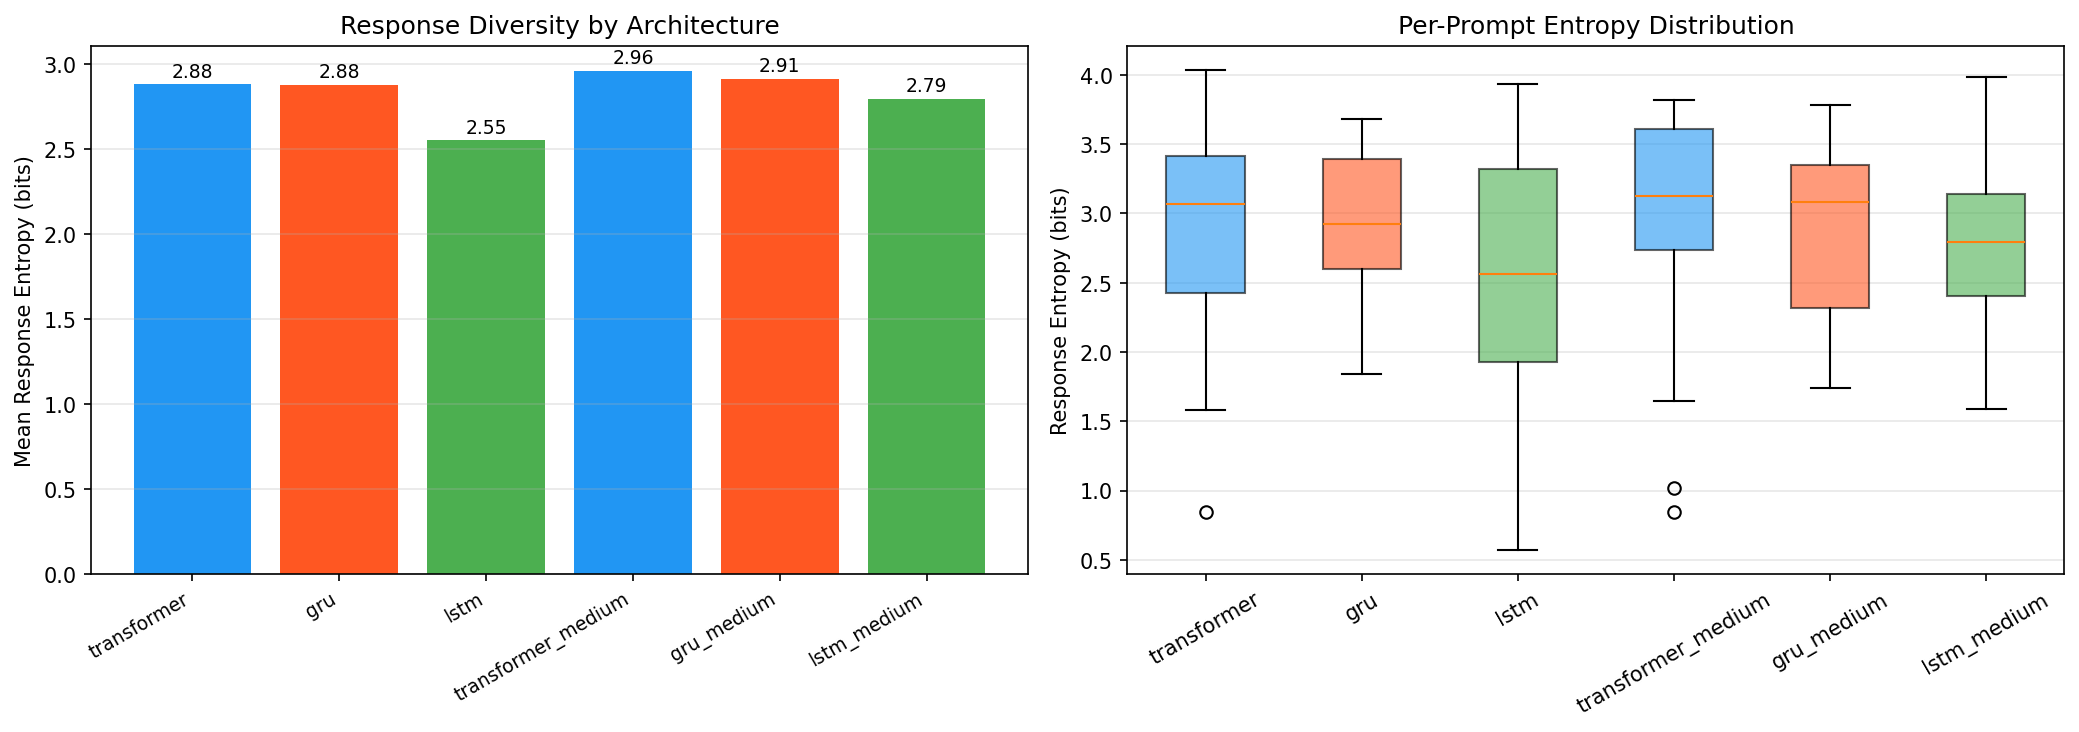
\includegraphics[width=0.95\linewidth]{figures/entropy_comparison.png}
\caption{Response entropy comparison across architectures. \transformer and \gru show comparable diversity, while \lstm produces less varied completions.}
\label{fig:entropy}
\end{figure}
